%!TEX root=seke.tex
% mainfile: ../seke.tex

% Box and whisker plots
% Belongs to results_bwplots, but must be here for positioning reasons

\begin{figure*}
\centering
\begin{subfigure}{0.5\textwidth}
  \centering
  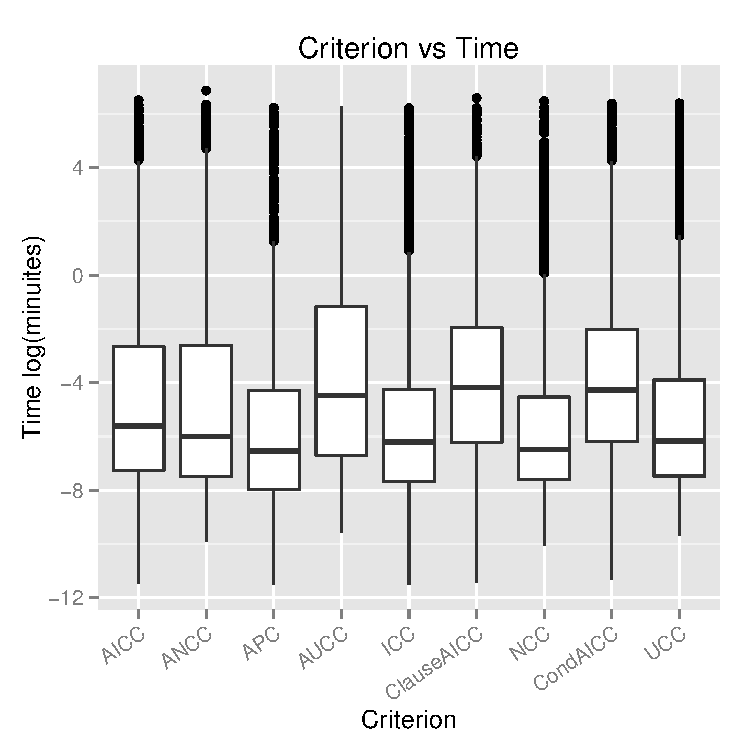
\includegraphics[width=1\linewidth]{diagrams/CriterionvsTime.pdf}
  \caption{Coverage criterion versus runtime in minutes.}
  \label{fig:crites}
\end{subfigure}%
\begin{subfigure}{0.5\textwidth}
  \centering
  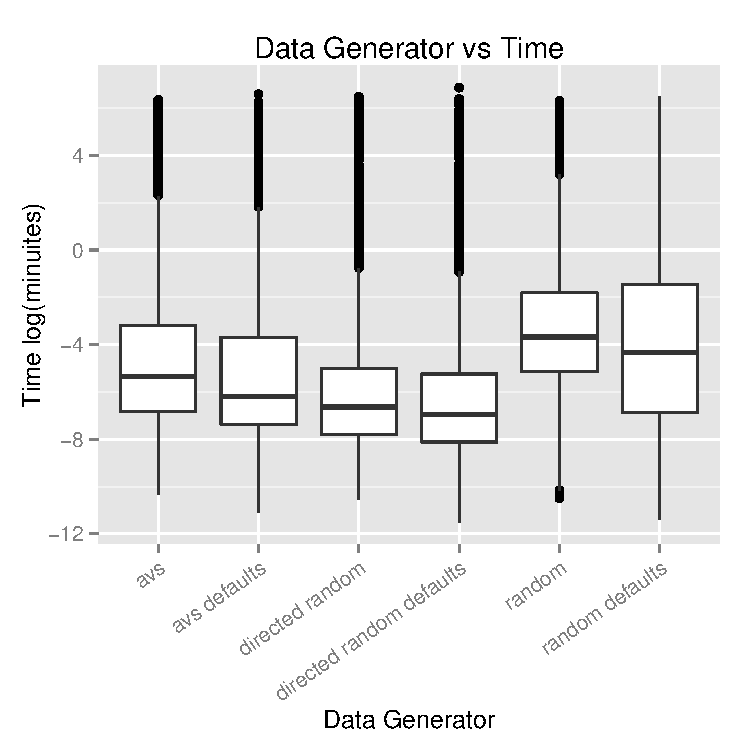
\includegraphics[width=1\linewidth]{diagrams/DataGeneratorvsTime.pdf}
  \caption{Data generator versus runtime in minutes.}
  \label{fig:datas}
\end{subfigure}
\label{fig:bwplots}
\caption{Box and whisker plots for criterion and data
  generator.}
\end{figure*}

To gain a more nuanced understanding of the results, we constructed a regression tree using the \textit{ctree} package
for the R langauge. A regression tree attempts to use the values of predictor variables to predict the value of a
responce variable. A regression tree accopmlishes this by repeadidily splitting the data according to what predictor
varaible has the most influcence on the response varaible. Each node in the tree represents a choice of predictor
varaible, and the level of the node indicates its importance to the prediction---higher being more important.

\textit{ctree} produced the tree shown as Figure~\ref{fig:atree} to predict the runtime of \textit{SchemaAnalyst} with
the predictor varaibles: tables, columns, {\tt UNIQUE}s, {\tt NOT NULL}s, {\tt CHECK}s, Criterion, and DataGenerator.
The regression tree confirms that the number of tables has the largest impact on runtime, and also reveals that when the
number of tables in the schema is small, the choice of coverage criterion is most significant.

While tables had a large impact when the number of tables was over 197 thousand, in practice schemas are unlikely to be
this large. Another invocation of \textit{ctree}, excluding tables from the list of predictors, provided insight into
the behavior of \textit{SchemaAnalyst} for more practical table sizes. Coverage criterion emereged as the most important
predictor for runtime, followed by the choice of data generator, and then the number of columns in the schema.
